\chapter{Development}

\section{Convolução e Convolução Discreta}
Em matemática, a convolução é um operador linear aplicado em duas funções. 
Uma operador linear, é um caso especifico de uma transformação linear, que por sua vez também pode ser chamada por mapeamento linear ou função linear, é uma operação que, dados os conjuntos não vazios $A$ e $B$, o mapeamento $f$ de $A$ para $B$ é denotador por $f : A \to B$ onde $A$ representa o domínio e $B$ representa a imagem.
Para um mapeamento dos espaços vetorias $A$ e $B$ sobre o mesmo corpo $C$ ser considerado linear, ele deve preservar as operações de adição vetorial e multiplicação por escalar. 
Ou seja, deve cumprir as seguinte condições:\\
(1) para qualquer vetor $a, a' \in A$, $f(a+a') = f(a) + f(a')$\\
(2) para qualquer número escalar $e$ e vetor $a \in A$, $f(ka) = kf(a)$\\
No caso especifico do operador linear, esta transformação deve ocorrer dentro de um mesmo espaço vetorial.
Ou seja, uma transformação $f$ em um espaço vetorial $A$ sobre um corpo $C$ representada por $f : A \to A$.
\citep{lipschutz2009linear} \\%\par
Dadas as definições anteriores, um operador linear $f$ em um espaço vetorial $R^2$, $f : R^2 \to R^2$, definido por $f(x,y) \to (x,-y)$, operando em cima de um vetor $a \in R^2$ tal que $a = (1,1)$, resulta em uma imagem de $a' = (1,-1)$, representados respectivamente pela linha azul e vermelha na figura \ref{fig:operacaolinear}.
\begin{figure}[h] 
  \centering
  \caption[Transformação Linear $f(x,y) \to (x,-y)$]{Transformação Linear $f(x,y) \to (x,-y)$}
    \label{fig:operacaolinear}
    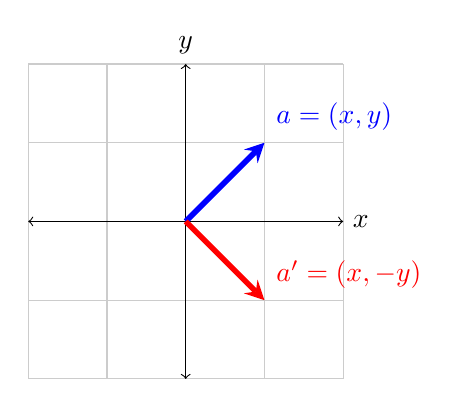
\begin{tikzpicture}
        \draw[thin,gray!40] (-2,-2) grid (2,2);
        \draw[<->] (-2,0)--(2,0) node[right]{$x$};
        \draw[<->] (0,-2)--(0,2) node[above]{$y$};
        \draw[line width=2pt,blue,-stealth](0,0)--(1,1) node[anchor=south west]{$\boldsymbol{a = (x,y)}$};
        \draw[line width=2pt,red,-stealth](0,0)--(1,-1) node[anchor=south west]{$\boldsymbol{a' = (x,-y)}$};
      \end{tikzpicture}
\end{figure}
Essa operação também pode ser representada de forma matricial. A transformação linear anteriormente denotada por $f(a)$ pode ser descrita pelo produto matricial da matriz de transformação $T : R^2 \in R^2$ pelo vetor $v$ tal que $v \in R^2$ da seguinte forma:
$$T = \begin{bmatrix}1 && 0 \\ 0 && -1\end{bmatrix} v = \begin{bmatrix}x \\ y\end{bmatrix}$$ 
$$T\cdot v = \begin{bmatrix}1 && 0 \\ 0 && -1\end{bmatrix}\begin{bmatrix}x \\ y\end{bmatrix} = \begin{bmatrix}x \\ -y\end{bmatrix}$$
Com os valores do vetor $v$ equivalentes ao vetor $a = (1,1)$ do exemplo anterior, temos a operação linear:
$$\begin{bmatrix}1 && 0 \\ 0 && -1\end{bmatrix}\begin{bmatrix}1 \\ 1\end{bmatrix} = \begin{bmatrix}1 \\ -1\end{bmatrix}$$






e produz uma terceira função que representa ... A convolução é uma operação matemática com aplicações em vários temas, e principalmente em processamento de sinais.


% \section{Introduction}

% \lipsum[1]

% \begin{code}[language=Python,caption=Python Fribonacci Code,label=code:frib]
% from math import *

% # define function
% def analytic_fibonacci(n):
%   sqrt_5 = sqrt(5);
%   p = (1 + sqrt_5) / 2;
%   q = 1/p;
%   return int( (p**n + q**n) / sqrt_5 + 0.5 )

% for i in range(1,31):
%   print analytic_fibonacci(i)
% \end{code}


% This is a reference to Code \ref{code:frib} \ldots{}

% \lipsum[1]

% \begin{code}[language=C,caption=Hello World C Code,label=code:helloc]
% #include<stdio.h>

% main()
%     {
%         printf("Hello World");
%     }
% \end{code}


% This is a reference to Code \ref{code:helloc} \ldots{}

% \lipsum[1]

% \begin{code}[language=Java,caption=Hello Java Code,label=code:helloj]
% public class HelloWorld {

%     public static void main(String[] args) {
%         System.out.println("Hello, World");
%     }
% }
% \end{code}


% This is a reference to Code \ref{code:helloj} \ldots{}


% \section{Section}

% \lipsum[2-4]

% \subsection{Subsection}

% \lipsum[2-4]
